\begin{frame}
\frametitle{Completed and future work}       
\begin{textblock*}{12.5cm}(0.1cm,2.2cm) % {block width} (coords)
	\begin{figure}[ht!] % replace 't' with 'b' to force it to 
		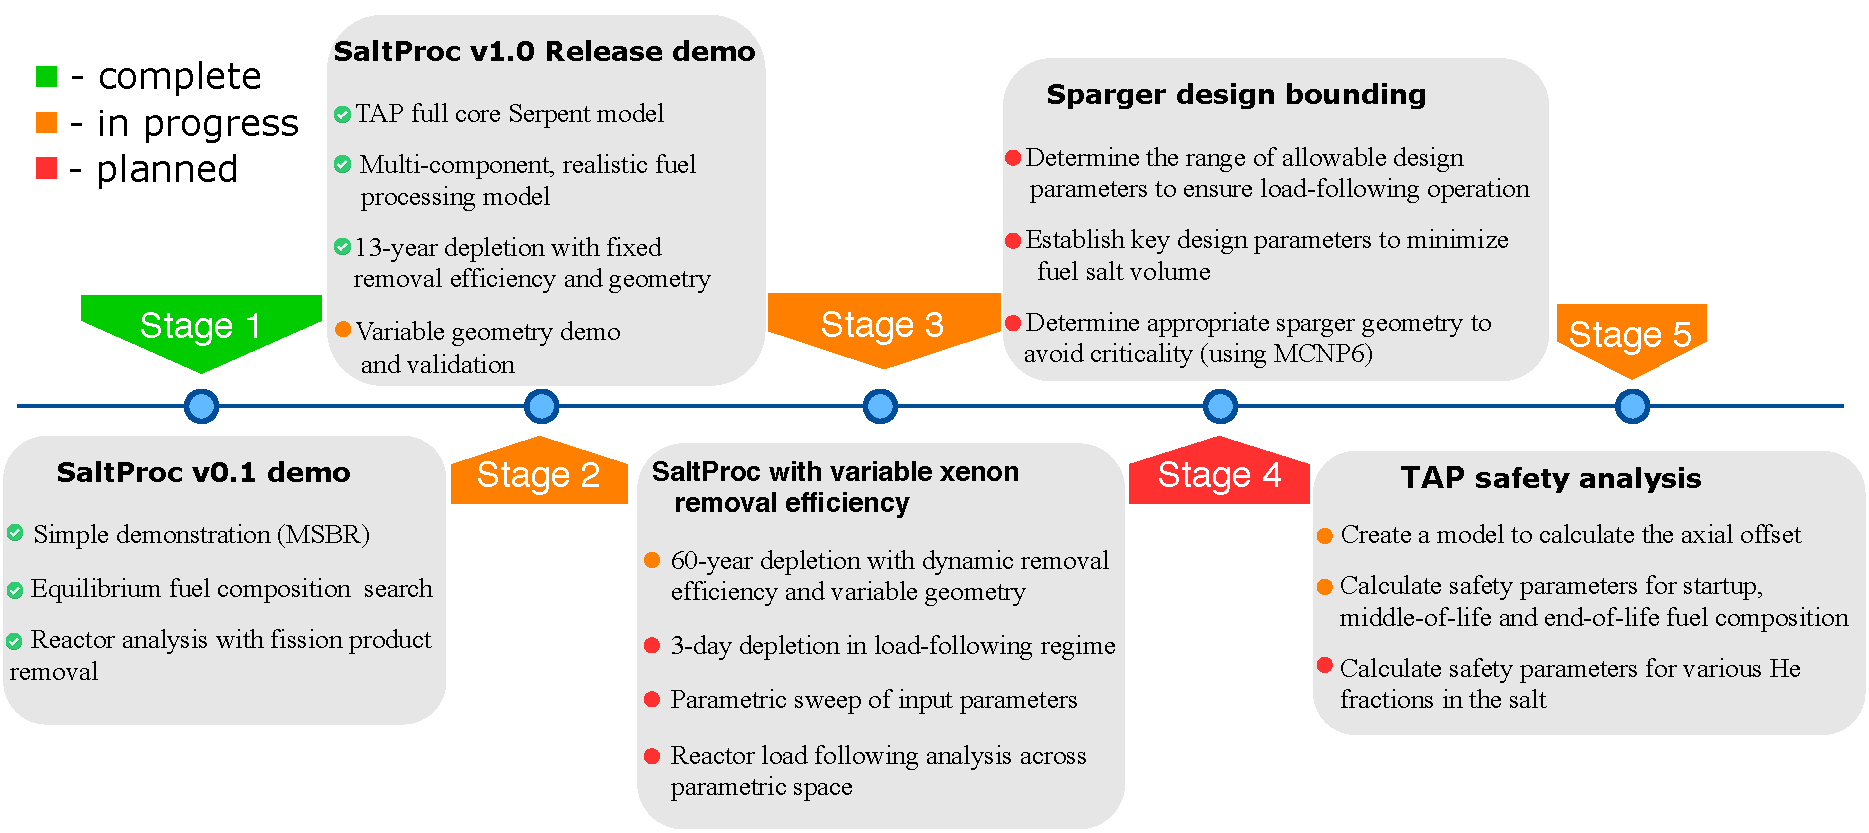
\includegraphics[width=\textwidth]{./images/progress_chart_larger.pdf} 
	\end{figure}
\end{textblock*}
\end{frame}

\begin{frame}
\frametitle{Conclusion}
	\begin{textblock*}{12cm}(0.4cm,2cm) % {block width} (coords)
	\begin{itemize}
		\itemsep1em
		\item Relevance
		\begin{itemize}
			\itemsep0.5em
			\item Fuel salt processing systems modeling in \glspl{MSR} based 
			on \textbf{many assumptions and estimations}
			\item This work will \textbf{more realistically} model salt 
			processing system with a \textbf{focus on the gas removal system}  
			of the prospective \gls{TAP} \gls{MSR}
		\end{itemize} 
		\item Preliminary results
			\begin{itemize}
				\itemsep0.5em
				\item Simple demonstration for \gls{MSBR} with 
				\textbf{ideal/fixed	fission products removal efficiency}
				\item \textbf{Multi-component} fuel reprocessing system 
				modeling with \textbf{non-ideal/constant} 
				efficiency
				\item \textbf{Effect of fission product removal} on the core 
				neutronics
			\end{itemize}
		
		\item Future work
			\begin{itemize}
				\itemsep0.5em
				\item Add \textbf{variable geometry} and \textbf{dynamic 
				removal efficiency capability}
				\item Demonstrate and validate those capabilities for 
				\textbf{lifetime-long depletion}
				\item Simulate short-term transients to determine the 
				\textbf{feasibility of load following}
				\item Determine feasible \textbf{design parameters of the 
				sparger}
				\item Analyze \textbf{dynamics of the safety parameters} for 
				long- and short-term cases
			\end{itemize}
	\end{itemize}
\end{textblock*}
\end{frame}

\begin{frame}
	\frametitle{Questions?}
\end{frame}